%!TEX program = xelatex

\documentclass[a4paper, openany, oneside]{memoir}
\usepackage[no-math]{fontspec}
\usepackage{pgfplots}
\pgfplotsset{compat=newest}
\usepackage{commath}
\usepackage{mathtools}
\usepackage{amssymb}
\usepackage{amsthm}
\usepackage{booktabs}
\usepackage{mathtools}
\usepackage{xcolor}
\usepackage[separate-uncertainty=true, per-mode=symbol]{siunitx}
\usepackage[noabbrev, capitalize]{cleveref}
\usepackage{listings}
\usepackage[american inductor, european resistor]{circuitikz}
\usepackage{amsmath}
\usepackage{amsfonts}
\usepackage{ifxetex}
\usepackage[dutch,english]{babel}
\usepackage[backend=bibtexu,texencoding=utf8,bibencoding=utf8,style=ieee,sortlocale=en_GB,language=auto]{biblatex}
\usepackage[strict,autostyle]{csquotes}
\usepackage{parskip}
\usepackage{import}
\usepackage{standalone}
\usepackage{hyperref}
%\usepackage[toc,title,titletoc]{appendix}

\ifxetex{} % Fonts laden in het geval dat je met Xetex compiled
    \usepackage{fontspec}
    \defaultfontfeatures{Ligatures=TeX} % To support LaTeX quoting style
    \setromanfont{Palatino Linotype} % Tover ergens in Font mapje in root.
    \setmonofont{Source Code Pro}
\else % Terug val in standaard pdflatex tool chain. Geen ondersteuning voor OTT fonts
    \usepackage[T1]{fontenc}
    \usepackage[utf8]{inputenc}
\fi
\newcommand{\references}[1]{\begin{flushright}{#1}\end{flushright}}
\renewcommand{\vec}[1]{\boldsymbol{\mathbf{#1}}}
\newcommand{\uvec}[1]{\boldsymbol{\hat{\vec{#1}}}}
\newcommand{\mat}[1]{\boldsymbol{\mathbf{#1}}}
\newcommand{\fasor}[1]{\boldsymbol{\tilde{\vec{#1}}}}
\newcommand{\cmplx}[0]{\mathrm{j}}
\renewcommand{\Re}[0]{\operatorname{Re}}
\newcommand{\Cov}{\operatorname{Cov}}
\newcommand{\Var}{\operatorname{Var}}
\newcommand{\proj}{\operatorname{proj}}
\newcommand{\Perp}{\operatorname{perp}}
\newcommand{\col}{\operatorname{col}}
\newcommand{\rect}{\operatorname{rect}}
\newcommand{\sinc}{\operatorname{sinc}}
\newcommand{\IT}{\operatorname{IT}}
\newcommand{\F}{\mathcal{F}}

\newtheorem{definition}{Definition}
\newtheorem{theorem}{Theorem}


\DeclareSIUnit{\voltampere}{VA} %apparent power
\DeclareSIUnit{\pii}{\ensuremath{\pi}}

\hypersetup{%setup hyperlinks
    colorlinks,
    citecolor=black,
    filecolor=black,
    linkcolor=black,
    urlcolor=black
}

% Example boxes
\usepackage{fancybox}
\usepackage{framed}
\usepackage{adjustbox}
\newenvironment{simpages}%
{\AtBeginEnvironment{itemize}{\parskip=0pt\parsep=0pt\partopsep=0pt}
\def\FrameCommand{\fboxsep=.5\FrameSep\shadowbox}\MakeFramed{\FrameRestore}}%
{\endMakeFramed}

% Impulse train
\DeclareFontFamily{U}{wncy}{}
\DeclareFontShape{U}{wncy}{m}{n}{<->wncyr10}{}
\DeclareSymbolFont{mcy}{U}{wncy}{m}{n}
\DeclareMathSymbol{\Sha}{\mathord}{mcy}{"58}
\addbibresource{../../includes/bibliography.bib}

\begin{document}
\section{Additional Analysis}

\subsection{Support of Solution}
Consider \cref{th:deci-corr}. Here $[E(N \vec{r}_{y'_i,y'_j})]_{m + L}$ is an estimator of $R_{Y'_i,Y'_j}[m]$ for $m = -L+1,L-1$. Since one is only able to estimate $R_{Y'_i,Y'_j}[m]$ for $m=-L+1,L-1$, it is often assumed that $R_{Y'_i,Y'_j}[m]=0$ for $m \le -L$ and $m \ge L$. But then $R_{Y'_i,Y'_j}[m]=0$ for $m \le -LN$ and $m \ge LN$, which implies that $E[(\vec{r}_{y_i,y_j})]_{m+LN + N-1}=0$ for $m \le -LN$ and $m \ge LN$. Therefore the first and last $N-1$ elements of $E[(\vec{r}_{y_i,y_j})]$ are zero. By the structure of $\mat{R}_{c_i,c_j}$, the first $N-1$ elements of $E(\vec{r}_x)$ consist of the first $N-1$ elements of $\vec{r}_{y_i,y_j}$, which are zero. Therefore, the first $N-1$ elements of $E(\vec{r}_x)$ are zero. Similarly, the last $N-1$ elements of $E(\vec{r}_x)$ are zero.

\subsection{Unicity of Solution}
rank => circ min sparse ruler

\subsection{Minimal Circular Rulers}
We introduce the concept of a ruler. Consider a ruler $\vec{r}$ of length $N$. Then $\vec{r} \in \{0,1\}^N$. Also, $(\vec{r})_i = 1$ if the element at position $i$ is marked, and $(\vec{r})_i = 0$ if the elements at position is not marked. We will formulate the minimal circular ruler problem as an binary integer linear program.

A ruler $\vec{r}$ contains a distance $d$ if there exist $i$ and $j$ such that $(\vec{r})_i = 1$, $(\vec{r})_j = 1$ and $|i-j| = d$ or  $N-|i-j| = d$. The ruler $\vec{r}$ is a circular ruler if it contains distances $ 1, \ldots, N - 1$. A circular ruler $\vec{r}$ is minimal if and only if $||\vec{r}||_1$ is minimal. A circular ruler can be depicted in a nice way. \Cref{fig:circular-ruler} shows a minimal circular ruler for $N=7$. The circle depicts the ruler and contains $N$ ticks. Then $(\vec{r})_i = 1$ if the tick at position $i$ is red. The definition of a circular ruler then states that the ruler is circular if and only if the distances between the marks are the distances $1,\ldots,N-1$.
\begin{figure}[H]
    \centering
    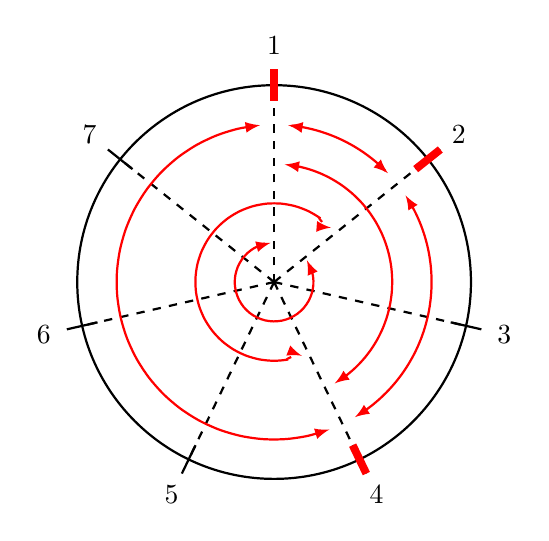
\begin{tikzpicture}
        \def\N{7}
        \draw [thick, black] circle[radius=2.5cm] (0,0);
        \foreach \i in {1,...,\N} {
            \draw [scale=1,domain=2.3:2.7,smooth,variable=\x,black,thick] plot ({\x*sin(360*(\i-1)/\N)},{\x*cos(360*(\i-1)/\N)});
            \draw [black,thick,dashed] (0,0) -- ({2.5*sin(360*(\i-1)/\N)},{2.5*cos(360*(\i-1)/\N)});
            \node[black] at ({3*sin(360*(\i-1)/\N)},{3*cos(360*(\i-1)/\N)}) {$\i$};
        }
        \foreach \i in {0,1,3} {
            \draw [scale=1,domain=2.3:2.7,smooth,variable=\x,red,line width=1mm] plot ({\x*sin(360*\i/\N)},{\x*cos(360*\i/\N)});
        }
        \draw [scale=1,domain=0.1:0.9,smooth,variable=\x,black,thick,>=latex,<->,red] plot ({2*sin(360*\x/\N)},{2*cos(360*\x/\N)}); % 1
        \draw [scale=1,domain=1.1:2.9,smooth,variable=\x,black,thick,>=latex,<->,red] plot ({2*sin(360*\x/\N)},{2*cos(360*\x/\N)}); % 2
        \draw [scale=1,domain=3.1:6.9,smooth,variable=\x,black,thick,>=latex,<->,red] plot ({2*sin(360*\x/\N)},{2*cos(360*\x/\N)}); % 4
        \draw [scale=1,domain=0.1:2.9,smooth,variable=\x,black,thick,>=latex,<->,red] plot ({1.5*sin(360*\x/\N)},{1.5*cos(360*\x/\N)}); % 3
        \draw [scale=1,domain=3.1:7.9,smooth,variable=\x,black,thick,>=latex,<->,red] plot ({1*sin(360*\x/\N)},{1*cos(360*\x/\N)}); % 5
        \draw [scale=1,domain=1.1:6.9,smooth,variable=\x,black,thick,>=latex,<->,red] plot ({0.5*sin(360*\x/\N)},{0.5*cos(360*\x/\N)}); % 6
    \end{tikzpicture}
    \caption{Minimal circular ruler for $N=7$}
    \label{fig:circular-ruler}
\end{figure}

\todo[inline, author=Kees]{Read from here}

\subsection{Optimal circular sparse rulers}
Let $\mathbf{S} \in \mathbb{N}^M$ with $S_i \leq N$ where $M$ is the amount of elements and $N$ the maximum length. We want this $\mathbf{S}$ to represent optimal circular sparse ruler solutions.

\begin{blockDefinition}
    Let $\mathbf{S} \in \mathbb{N}^M$ , then the set of lags $\Omega = \{|n_i-n_j|\} \cup \{N-|n_i-n_j|\} \quad \forall_{n_i,n_j}\in \mathbf{S}$.
\end{blockDefinition}
    

\begin{blockDefinition}
    $\mathbf{S}$ is an optimal circular sparse ruler solution if $\mathbf{S}$ is a circular sparse ruler solution, and there exists no circular sparse ruler solution with greater length while having the same amount of elements.
\end{blockDefinition}

\subsection{Verifying circular sparse rulers}

\begin{blockTheorem} \label{th:circ_verify}\nolinebreak
    $\mathbf{S}$ is a solution of circular sparse ruler if and only if all lags $\{0,1,\dots, \lfloor\frac{N}{2}\rfloor\}$ can be made. \nolinebreak
\end{blockTheorem}

\begin{blockProofTheorem}{\ref{th:circ_verify}}
    Given lag $k$, one can get lag $N-k$ by turning in opposite direction on the circle. Assume that $\mathbf{S}$ contains all lags $\{0,1,\dots, A\}$. It then follows that one can also make the lags  $\{N-A,N-A+1,\dots, N-1\}$. If $(N-A)-A \leq 1$ then the two sets of lags connect to the set of lags $\{0,1,\dots,N-1\}$. $A=\lfloor\frac{N}{2}\rfloor$. $N-\lfloor\frac{2N}{2}\rfloor \leq 1$.
\end{blockProofTheorem}

\subsection{Circular sparse ruler from optimal linear sparse ruler}\label{ssec:minimal_linear_s}
Linear sparse ruler is a problem that is already well defined and researched. 

\begin{blockDefinition}\label{def:minimal_sparse}
    $\mathbf{S}$ is a minimal linear sparse ruler solution of length $N$ if 
    $$
    \min_S|S| \quad s.t. \{0,1,\dots,N-1\} \in \Omega_{\text{linear}}
    $$
\end{blockDefinition}

From definition \ref{def:minimal_sparse} one can see that a minimal sparse ruler solution guarantees a set where $\{0,1,\dots,N_{linear}-1\} \in \Omega$. We can use theorem \ref{th:circ_verify} to show that the minimal sparse ruler solution with length $N_{linear}$ is also a solution for circular sparse ruler with $N=2N_{linear}-1$.
For example, the minimal sparse ruler solution for $N_{linear}=7$: $\{1,2,5,7\}$ is also a valid circular sparse ruler solution for $N=13$.

\subsection{Upper-bound and lower-bound of optimal circular sparse ruler}
To tell whether a circular sparse ruler solution is also optimal, it is useful to define an upper and lower-bound. The lower-bound is the minimal optimal solution one can get with $M$ elements. For this we can simply use the minimal linear sparse ruler solutions as described in section \ref{ssec:minimal_linear_s}, because this allows us to easily find circular sparse ruler solutions. The upper bound is the theoretical maximum amount of length $N$ one can achieve with $M$ elements.

\begin{blockTheorem} \label{th:upperbound}\nolinebreak
    the maximum length $N$ one can achieve with $M$ elements is $N=M(M-1)+1$\nolinebreak
\end{blockTheorem}

\begin{blockProofTheorem}{\ref{th:upperbound}}
    Let $\mathbf{S} \in \mathbb{N}^M$, and $n_i,n_j \in \mathbf{S}$, then the amount of lags $\Omega$ one can make with $M$ elements is $M^2$. We are only interested in unique combinations. Out of the $M^2$ combinations $M$ are $n_i=n_j$, resulting in a lag of 0. These cannot be unique, so the theoretic maximum amount of unique lags is reduced to $N=M(M-1)+1$
\end{blockProofTheorem}

\subsection{The structure of optimal circular sparse rulers}

\begin{blockTheorem} \label{th:lag1}\nolinebreak
    Let $M$ be the amount of elements and $N$ the length of a solution $\mathbf{S}$, and $M\geq 2$, then there exists a solution $\mathbf{S}$ with the same $M$ and $N$ where $\{1,2\} \in \mathbf{S}$  \nolinebreak
\end{blockTheorem}

\begin{blockProofTheorem}{\ref{th:lag1}}
    For every solution holds: $1 \in \Omega$. Therefore there are always two elements next to each other. Because the problem is circular, one can translate the locations of the elements freely. Therefore one can always get a solution where $\{1,2\} \in \mathbf{S}$
\end{blockProofTheorem}

This is a useful property when writing an algorithm, for it allows the first two elements to be forced.



\begin{blockTheorem} \label{th:lag2}\nolinebreak
    all circular sparse ruler solutions can be written as $\{1,2,3\} \in \mathbf{S}$, $\{1,2,4\} \in \mathbf{S}$,  or $\{1,2,k, k+2\} \in \mathbf{S}$ where $k \in \{5,6,\dots,\lfloor\frac{N}{2}\rfloor-1\}$, or a rotation of those. \todo{dit is net niet lekker geformuleerd}   \nolinebreak
\end{blockTheorem}

\begin{blockProofTheorem}{\ref{th:identical_lags}}
    We know that lag $2 \in \Omega$, therefore there need to be two devices with distance two from each other. This can be done in combination with element 1 or 2 from theorem \ref{th:lag1}. The only way to achieve this is $\{1,2,3\} \in \mathbf{S}$, $\{1,2,4\}$, $\{1,2,N\}$, $\{1,2,N-1\}$, but the last two options are identical to the first two except for their rotation. If no combination with element 1 or 2 is used then two other devices must be somewhere with distance 2 from each other. All options can be covered with $\{1,2,k, k+2\} \in \mathbf{S}$ where $k \in \{5,6,\dots,N-4\}$, but this set can also be reduced by exploiting rotation, resulting in $\{1,2,k, k+2\} \in \mathbf{S}$ where $k \in \{5,6,\dots,\lfloor\frac{N}{2}\rfloor-1\}$. Therefore every solution can be written as $\{1,2,3\} \in \mathbf{S}$, $\{1,2,4\} \in \mathbf{S}$,  or $\{1,2,k, k+2\} \in \mathbf{S}$ where $k \in \{5,6,\dots,\lfloor\frac{N}{2}\rfloor-1\}$, or a rotation of those. 
\end{blockProofTheorem}

This theorem has the potential to be used for a substantial speed-up when designing an algorithm.

\begin{blockTheorem} \label{th:identical_lags}\nolinebreak
    Let $\mathbf{S}$ be a solution to minimal circular sparse ruler. The amount of identical lags in $\Omega$ are $N_{\text{lags}} = M(M-1)+1-N$   \nolinebreak
\end{blockTheorem}

\begin{blockProofTheorem}{\ref{th:identical_lags}}
    For a given $M$ elements there are $M(M-1)+1$ different combination possible. See theorem \ref{th:upperbound}. The amount of different lags in a solution is $N$. Therefore the amount of identical lags is $N_{\text{lags}} = M(M-1)+1-N$ 
\end{blockProofTheorem}

\subsection{Guesswork}
\todo{Guesswork? Wat is de engelse variant van een vermoeden?}

\begin{blockTheorem} \label{th:odd}\nolinebreak
    The length $N$ of an optimal solution $\mathbf{S}$ is an odd integer \nolinebreak
\end{blockTheorem}

This is something that has no proof yet, but holds some intuition to it. One wants to optimize the amount of different lags. When $N$ is even, there  needs to be a lag $|\frac{N}{2}|$, but when there is such a lag one also has the lag $N-|\frac{N}{2}|=|\frac{N}{2}|$. So with $N$ is even, one always has a double lag. Also the trend in the solution set for $2<N<40$ supports this. The minimal circular sparse ruler for $N=38$ has $M=8$, while the minimal sparse ruler for $N=39$ has $M=7$. Therefore the theorem \ref{th:odd} is a good assumption when writing an algorithm.

\begin{blockTheorem} \label{th:lag1_2}\nolinebreak
    Let $M$ be the elements and $N$ the length of an minimal circular sparse ruler solution, then there exists a solution $\mathbf{S}$ with these properties where lag 1 and 2 are only achieved with one combination   \nolinebreak
\end{blockTheorem}

This theorem also has no proof yet, but it also holds some intuition. A solution is optimal when it has as few identical lags as possible. If this theorem should be false then there would be a minimal solution where either lag 1 or lag 2 are double, but when lag 1 and 2 are double, that means that there are at least 6 double lags. Looking at theorem \ref{th:identical_lags} this performance is unacceptable for low $M$. Additional work needs to be done to prove this theorem, but it can already be used as an assumption to search for circular sparse ruler solutions quicker.

\subsection{Recursive algorithm}
Assuming all theorems above are correct, one can make an algorithm that quickly searches for circular sparse ruler solutions. Some additional work needs to be done to describe this algorithm.

\subsection{A set of optimal circular sparse rulers}
\begin{align}
M=2,N=3  \quad S&=\{1,2\}\\
M=3,N=7  \quad S&=\{1,2,4\}\\
M=4,N=13 \quad S&=\{1,2,5,7\}\\
M=5,N=21 \quad S&=\{1,2,7,9, 19\}\\
M=6,N=31 \quad S&=\{1,2,5,7,14,22\}\\
M=7,N=39 \quad S&=\{1,2,5,7,14,21,31\}
\end{align}

\todo[inline, author=Kees]{Read until here}

\begin{blockDefinition}
    Let $\vec{x} \in \{1\}^N$. Then $\vec{1}_N$ denotes $\vec{x}$.
\end{blockDefinition}

Let $D_d$ be the set consisting of the vectors $\vec{d} \in \{0,1\}^N$ such that $(\vec{d})_i=1$ and $(\vec{d})_{i+d}=1$ where $i = 1,\ldots,N-d$ or $(\vec{d})_i=1$ and $(\vec{d})_{i+d-N}$ where $i = N-d+1,\ldots,N-1$.
% \begin{align*}
%     D_d = \{\vec{d} \in \{0,1\}^N : (\vec{d})_i = 1, (\vec{d})_{i + d} = 1, i = 1,\ldots,N-d~\}~\cup \pushline \pushright{\{\vec{d} \in \{0,1\}^N : (\vec{d})_i = 1, (\vec{d})_{i + d - N} = 1, i = N-d+1,\ldots,N-1\}}
% \end{align*}
% for $d = 1,\ldots,N-1$.
We now formulate a theorem which guarantees that a ruler contains a specific distance.

\begin{blockTheorem} \label{th:ruler-distance}\nolinebreak
    Let $\vec{r} \in \{0,1\}^N$ be a ruler. Then $\vec{r}$ contains the distance $d$ if $\vec{d}^T \vec{r} = 2$ for any $\vec{d} \in D_d$.\nolinebreak
\end{blockTheorem}

\begin{blockProofTheorem}{\ref{th:ruler-distance}}
    Assume that $\vec{d}^T\vec{r} = 2$. Then there exist $i$ and $j$ such that $(\vec{d})_i (\vec{r})_i + (\vec{d})_j (\vec{r})_j = 2$. This implies that $(\vec{r})_i = 1$ and $(\vec{r})_j = 1$. Since $\vec{d} \in D_d$, either $|i-j|=d$ or $|i-j| = N-d$. In both cases, $\vec{r}$ contains the distance $d$. 
\end{blockProofTheorem}

Let $\mat{D}_d$ denote the $|D_d| \times N$ matrix which contains all vectors in $D_d$ as rows.

\begin{blockTheorem} \label{th:ruler-distance-matrix}\nolinebreak
    Let $\vec{r} \in \{0,1\}^N$ be a ruler and let $\vec{y} \in \{0,1\}^{|D_d|}$. Then $\vec{r}$ contains the distance $d$ at least once if $\mat{D}_d \vec{r} \ge 2\vec{y}$ such that $||\vec{y}||_1 = 1$.
\end{blockTheorem}

\begin{blockProofTheorem}{\ref{th:ruler-distance-matrix}}
    Assume that $\mat{D}_d \vec{r} \ge 2 \vec{y}$ such that $||\vec{y}||_1 = 1$. Then there is one and only one $i$ such that $(\vec{y})_i=1$. Therefore there exists a $\vec{d} \in D_d$ such that $\vec{d}^T \vec{r} \ge 2 (\vec{y})_i = 2$. Since $||\vec{d}||_1=2$, the equality holds and thus $\vec{r}$ contains the distance $d$. Now consider $\vec{d}' \in D_d$ such that $\vec{d}' \neq \vec{d}$. Then $\vec{d}^T \vec{r} \ge 0$, which holds for any $\vec{r}$.  
\end{blockProofTheorem}

Consider the binary integer linear program
\begin{align*}
    \text{minimise } &\vec{1}_N^T \vec{r} \\
    \text{such that } &
    \begin{bmatrix}
        \mat{D}_1 \\
        \vdots \\
        \mat{D}_{N-1}
    \end{bmatrix} \vec{r} \ge 2 \begin{bmatrix}
        \vec{y}_1 \\
        \vdots \\
        \vec{y}_2
    \end{bmatrix}, \begin{bmatrix}
        \vec{1}_{|D_1|}^T & & \\
        & \ddots & \\
        & & \vec{1}_{|D_{N-1}|}^T
    \end{bmatrix}  \begin{bmatrix}
        \vec{y}_1 \\
        \vdots \\
        \vec{y}_{N-1}
    \end{bmatrix} = \vec{1}_{N-1}, \\
    & \vec{r} \in \{0,1\}^N \text{ and } \vec{y}_i \in \{0,1\}^{|D_i|} \text{ for } i = 1,\ldots,N-1.
\end{align*}
Then, by the definition of a minimal circular ruler and \cref{th:ruler-distance-matrix}, this program yields a minimal circular ruler of length $N$.

\subsection{Oversampling}
Let $K \in \mathbb{N}$ denote the oversampling factor. Instead of obtaining $L$ samples from each coset to estimate all correlations from $-L+1$ to $L-1$, we could use $KL$ samples to estimate all correlations from $-L+1$ to $L-1$.

Consider \cref{th:deci-corr}. Let $\vec{z}'_i, \vec{z}'_j \in \mathbb{C}^{KL}$ denote the samples obtained by cosets $i$ and $j$ such that $(\vec{z}'_i)_m = Y'_i[m]$ and $(\vec{z}'_j)_m=Y'_j[m]$ for $m = 1,\ldots,KL$. Then note that $\vec{z}'_i[1,L]=\vec{y}'_i$ and $\vec{z}'_j[1,L]=\vec{y}'_j$. Let $\vec{r}_{z'_i,z'_j} = \vec{z}'_i \circ \vec{z}'_j$. Furthermore, let $r_z[n]$ denote a discrete signal such that $r_z[m] = (\vec{r}_{z'_i,z'_j})_{m+KL}$ for $m = -KL+1,\ldots,KL-1$. Then
\begin{align*}
    E(r_z[m]) = W_z[m]R_{Y'_i,Y'_j}[m]
\end{align*}
where
\begin{align*}
    W_z[m] = \begin{cases}
        m + KL & \text{if } -KL + 1 \le m \le 0, \\
        KL - m & \text{if } 0 \le m \le KL - 1, \\
        0 & \text{elsewhere.}
    \end{cases}
\end{align*}
Also, let $r_y[n]$ denote a discrete signal such that $r_y[m] = (\vec{r}_{y'_i,y'_j})_{m+L}$ for $m = -L+1,\ldots,L-1$. Then
\begin{align*}
    E(r_y[m]) = W_y[m]R_{Y'_i,Y'_j}[m]
\end{align*}
where
\begin{align*}
    W_y[m] = \begin{cases}
        m + L & \text{if } -L+1 \le m \le 0, \\
        L - m & \text{if } 0 \le m \le L - 1, \\
        0 & \text{elsewhere.}
    \end{cases}
\end{align*}
Ideally, we would want to use $r_z[m]$ to estimate $E(r_y[m])$ for $m = -L+1,\ldots,L-1$. This can be done by introducing
\begin{align*}
    W_{z \to y}[m] = \begin{cases}
        (m + L)/(m + KL) & \text{if } -L+1 \le m \le 0, \\
        (L - m)/(KL - m) & \text{if } 0 \le m \le L - 1, \\
        0 & \text{elsewhere.}
    \end{cases}
\end{align*}
$W_{z \to y}$ transforms the window applied by $r_y[m]$ to the window applied by $r_z[m]$ to prevent biasing. This is pictured by the green arrows in \cref{fig:window}.

\begin{figure}[H]
    \centering
    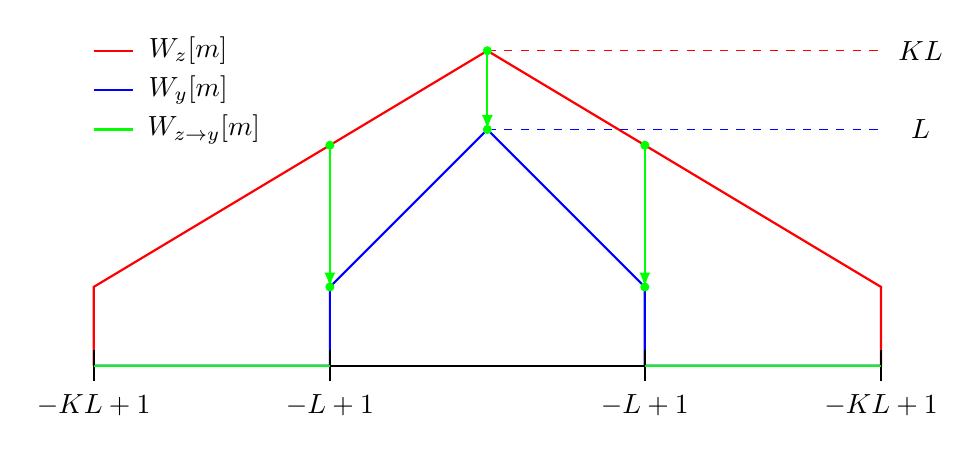
\begin{tikzpicture}
        \draw [red, thick] (-5, -1) -- (-5, 0) -- (0, 3) -- (5, 0) -- (5, -1);
        \draw [blue, thick] (-5, -1) -- (-2, -1) -- (-2, 0) -- (0, 2) -- (2, 0) -- (2, -1) -- (5, -1);
        \draw [blue, dashed] (0, 2) -- (5, 2);
        \draw (5, 2) node[black, xshift=0.5cm] {$L$};
        \draw (5,3) node[black, xshift=0.5cm] {$KL$};
        \draw [red, dashed] (0, 3) -- (5, 3);
        \draw [black, thick] (-5, -1) -- (5, -1);
        \draw [black, thick] (-5, -1.2) -- (-5, -0.8);
        \draw [black, thick] (-2, -1.2) -- (-2, -0.8);
        \draw [black, thick] (5, -1.2) -- (5, -0.8);
        \draw [black, thick] (2, -1.2) -- (2, -0.8);
        \draw (-5, -1) node[black, yshift=-0.5cm] {$-KL+1$};
        \draw (-2, -1) node[black, yshift=-0.5cm] {$-L+1$};
        \draw (5, -1) node[black, yshift=-0.5cm] {$-KL+1$};
        \draw (2, -1) node[black, yshift=-0.5cm] {$-L+1$};
        \draw [>=latex, ->, green, thick] (0, 3) to (0, 2);
        \draw [green, fill=green] (0, 3) circle [radius=0.05];
        \draw [green, fill=green] (0, 2) circle [radius=0.05];
        \draw [>=latex, ->, green, thick] (2, 1.8) to (2, 0);
        \draw [green, fill=green] (-2, 1.8) circle [radius=0.05];
        \draw [green, fill=green] (2, 1.8) circle [radius=0.05];
        \draw [green, fill=green] (-2, 0) circle [radius=0.05];
        \draw [>=latex, ->, green, thick] (-2, 1.8) to (-2, 0);
        \draw [green, fill=green] (2, 0) circle [radius=0.05];
        \draw [green, thick] (2, -1) -- (5, -1);
        \draw [green, thick] (-2, -1) -- (-5, -1);
        %\draw [green, thick, >=latex, ->] (-3.6, 0.6) to[bend left=25] (-3, -0.8);

        \draw [red, thick] (-5,3) -- (-4.5,3);
        \draw (-4.5,3) node[black, xshift=0.7cm] {$W_z[m]$};
        \draw [blue, thick] (-5,2.5) -- (-4.5,2.5);
        \draw (-4.5,2.5) node[black, xshift=0.7cm] {$W_y[m]$};
        \draw [green, thick] (-5,2) -- (-4.5,2);
        \draw (-4.5,2) node[black, xshift=0.9cm] {$W_{z \to y}[m]$};
    \end{tikzpicture}
    \caption{Transformation of the window applied by $r_y[m]$}
    \label{fig:window}
\end{figure}

Then
\begin{align*}
    E(W_{z \to y}[m]r_z[m]) &= W_{z \to y}[m] W_z[m] R_{Y'_i,Y'_j}[m] \\
    &= W_y[m] R_{Y'_i,Y'_j}[m] \\
    &= E(r_y[m]).
\end{align*}
To this end, let $\vec{w}_{z \to y} \in \mathbb{C}^{2L-1}$ be such that $(\vec{w}_{z \to y})_{i+L} = W_{z \to y}[i]$ for $i = -L+1,\ldots,L-1$. Then
\begin{align*}
    \vec{w}_{z \to y} =\begin{bmatrix}
        \frac{1}{KL - L + 1} & \cdots & \frac{L- 1}{KL - 1} & K & \frac{L- 1}{KL - 1} & \cdots & \frac{1}{KL - L + 1}
    \end{bmatrix}^T.
\end{align*} 
We can now state that
\begin{align*}
    E(N \vec{r}_{z'_i,z'_j}[KL-L+1,KL+L-1] \odot \vec{w}_{z \to y}) = E(N \vec{r}_{y'_i,y'_j}) = E(\vec{r}'_{y_i,y_j}).
\end{align*}
Thus
\begin{align*}
    \vec{r}'_y = N\begin{bmatrix}
        \vec{r}_{z'_1,z'_1}[KL-L+1,KL+L-1] \\
        \vdots \\
        \vec{r}_{z'_M,z'_M}[KL-L+1,KL+L-1]
    \end{bmatrix} \odot \begin{bmatrix}
        \vec{w}_{z \to y} \\
        \vdots \\
        \vec{w}_{z \to y} 
    \end{bmatrix}
\end{align*}
could be used instead.

TODO: Argue that using oversampling decreases mean squared error. And that $\vec{w}_{z\to y}$ slightly increases mean squared error, but makes the estimation unbiased (already shown).


\subsection{Sample-Wide Autocorrelation}
TODO: Revise

Is it possible to estimate $E(\vec{r}_x)$ by making use of $\vec{w}_m$. To this end,
\begin{align*}
    (\vec{w}_m \circ \vec{w}_m)_i &= \sum_{k=1}^M (\vec{w}_m)_k (\conj{\vec{w}}_m)_{M-i+k} \\
    &= \sum_{k=1}^M (\vec{d}_k^T \vec{x}_m)(\conj{\vec{d}}_{M-i+k}^T \conj{\vec{x}}_m) \\
    &= \sum_{k=1}^M (\vec{x}_m^T \vec{d}_k)(\conj{\vec{d}}_{M-i+k}^T \conj{\vec{x}}_m)
\end{align*}
where $\vec{d}_i = \vec{0}$ for $i < 1$ and $i > M$. Let
\begin{align*}
     \mat{A}_i = \sum_{k=1}^M  \vec{d}_k \conj{\vec{d}}_{M-i+k}^T
\end{align*}
for $i = 1,\ldots,2M-1$. Then
\begin{align*}
    (\vec{w}_m \circ \vec{w}_m)_i &= \sum_{k=1}^M \vec{x}_m^T (\vec{d}_k \conj{\vec{d}}_{M-i+k}^T) \conj{\vec{x}}_m \\
    &= \vec{x}_m^T\left(\sum_{k=1}^M  \vec{d}_k \conj{\vec{d}}_{M-i+k}^T\right) \conj{\vec{x}}_m \\
    &= \vec{x}_m^T \mat{A}_i \conj{\vec{x}}_m \\
    &= \sum_{k = 1}^N \sum_{l=1}^N (\vec{x}_m)_k (\conj{\vec{x}}_m)_l (\mat{A}_i)_{k,l} \\
    &= \sum_{k = 1}^N \sum_{l=1}^N (\vec{x})_{(m-1)N+k} (\conj{\vec{x}})_{(m-1)N+l} (\mat{A}_i)_{k,l}.
\end{align*}
Now let $\vec{\mathfrak{x}} \in \mathbb{C}^{(LN)^2}$ be such that $(\vec{\mathfrak{x}})_{(i-1)LN+j} = (\vec{x})_i (\conj{\vec{x}})_j$ for $i = 1,\ldots,LN$ and $j = 1,\ldots,LN$. Then
\begin{align*}
    (\vec{w}_m \circ \vec{w}_m)_i = \vec{p}_{m,i}^T \vec{\mathfrak{x}}
\end{align*}
where $\vec{p}_{m,i} \in \mathbb{C}^{(LN)^2}$ such that
\begin{align*}
    (\vec{p}_{m,i})_{[(m-1)N+k-1]LN+(m-1)N+l} = (\mat{A}_i)_{k,l}
\end{align*}
for $k = 1,\ldots,N$ and $l = 1,\ldots,N$. Now let $\vec{r}_w$ and $\mat{P}$ be such that
\begin{align*}
    \vec{r}_w = \begin{bmatrix}
        (\vec{w}_1 \circ \vec{w}_1)_1 \\
        \vdots \\
        (\vec{w}_L \circ \vec{w}_L)_{2M-1}
    \end{bmatrix} = \begin{bmatrix}
        \vec{p}_{1,1}^T \vec{\mathfrak{x}} \\
        \vdots \\
        \vec{p}_{L,2M-1}^T \vec{\mathfrak{x}}
    \end{bmatrix} = \begin{bmatrix}
        \vec{p}_{1,1}^T \\
        \vdots \\
        \vec{p}_{L,2M-1}^T
    \end{bmatrix} \vec{\mathfrak{x}} = \mat{P} \vec{\mathfrak{x}}.
\end{align*}
Similarly, we can relate
\begin{align*}
    (\vec{r}_x)_i &= \sum_{k=1}^{LN}(\vec{x})_k (\conj{\vec{x}})_{LN-i+k} \\
    &= \vec{b}_i^T \vec{\mathfrak{x}}
\end{align*}
where $\vec{b}_i \in \mathbb{C}^{(LN)^2}$ is such that
\begin{align*}
    (\vec{b}_i)_{(k-1)LN+LN-i+k} = 1
\end{align*}
for $k = 1,\ldots,LN$ such that $1 \le LN-i+k \le LN$. Now let $\mat{B}$ be such that
\begin{align*}
    \vec{r}_x = \begin{bmatrix}
        (\vec{r}_x)_1 \\
        \vdots \\
        (\vec{r}_x)_{2LN-1}
    \end{bmatrix} = \begin{bmatrix}
        \vec{b}_1^T \vec{\mathfrak{x}} \\
        \vdots \\
        \vec{b}_{2LN-1}^T \vec{\mathfrak{x}}
    \end{bmatrix} = \begin{bmatrix}
        \vec{b}_1^T \\
        \vdots \\
        \vec{b}_{2LN-1}^T
    \end{bmatrix} \vec{\mathfrak{x}} = \mat{B} \vec{\mathfrak{x}}.
\end{align*}
This yields the system
\begin{align*}
    \vec{r}_w &= \mat{P} \vec{\mathfrak{x}}, \\
    \vec{r}_x &= \mat{B} \vec{\mathfrak{x}}
\end{align*}
which can be used in a similar way to estimate $E(\vec{r}_x)$. However, since $\mat{A}_i$ is an $N \times N$ matrix, all elements in $\vec{p}_{m,i}$ relating to $(\vec{x})_k (\conj{\vec{x}})_l$ where $|k - l| \ge N$ will be zero. Therefore using $\vec{r}_w$ to estimate $E(\vec{r}_x)$ yields that the estimation is limited in support from $-N+1$ to $N-1$. This damages the resolution severely.

\subsection{Discussion of \cref{th:corr-unbiased}}
In this section we discuss the applicability of \cref{th:corr-unbiased} on the algorithm. Let $r[n]$ be a discrete signal such that $r[i] = (\vec{r}_x)_{i+LN}$ for $i = -LN+1,\ldots,LN-1$. Then
\begin{align*}
    E(r[i])=E[(\vec{r}_x)_{i + LN}]=W[i]R_X[i]
\end{align*}
where
\begin{align*}
    W[i] = \begin{cases}
        i+LN  &\text{if } -LN+1 \le i \le 0, \\
        LN-i&\text{if } 0 \le i \le LN-1, \\
        0 & \text{elsewhere.}
    \end{cases}
\end{align*}

First, one could propose to use $(W[i])^{-1}E(r[i])$ as an unbiased estimator of $R_X[i]$ for $i=-LN+1,\ldots,LN-1$. However, \cite{percival1993univariate} shows that this usually increases the mean squared error.

Second, $E(\vec{r}_x)$ is usually estimated to estimate the power spectral density of $X[n]$. Therefore, we study the effect of $W[n]$ on the power spectral density. By the convolution theorem and the Wiener-Khintchine theorem,
\begin{align*}
    \DTFT\{E(r[i])\} = \frac{1}{2 \pi}\DTFT\{R_X[i]\} \circledast \DTFT\{W[i]\} = \frac{1}{2 \pi}\mathcal{P}(\omega) \circledast \DTFT\{W[i]\}
\end{align*}
where $\mathcal{P}(\omega)$ denotes the power spectral density of $X[n]$. Note that
\begin{align*}
    \DTFT\{W[i]\} &= \sum_{k=-\infty}^{\infty}W[k]\exp(-j \omega k) \\
    &= \sum_{k=-LN+1}^{0}(k +LN)\exp(-j \omega k) + \sum_{k=1}^{LN-1}(LN-k) \exp(-j \omega k) \\
    &= \sum_{k=0}^{LN-1} \left[(LN-k) \exp(j \omega k) + (LN-k) \exp(-j \omega k) \right] - LN \\
    &= \sum_{k=0}^{LN-1} \left[\left(LN+j\frac{d}{d \omega}\right) \exp(j \omega k) \right. \\
    \pushright{\left. + \left(LN-j \frac{d}{d \omega}\right) \exp(-j \omega k) \right] - LN} 
    &= \left(LN+j\frac{d}{d \omega}\right) \sum_{k=0}^{LN-1}\exp(j \omega k) \\
    \pushright{+ \left(LN-j \frac{d}{d \omega}\right) \sum_{k=0}^{LN-1} \exp(-j \omega k) - LN}
    &= \left(LN+j\frac{d}{d \omega}\right) \frac{1-\exp(j \omega LN)}{1-\exp(j \omega)}
    \pushright{+ \left(LN-j \frac{d}{d \omega}\right) \frac{1-\exp(-j \omega LN)}{1-\exp(-j \omega)} - LN.} 
\end{align*}
Further algebraic simplification yields that
\begin{align*}
    \DTFT\{W[i]\} = \frac{\cos(LN \omega) - 1}{\cos(\omega) - 1}.
\end{align*}
Since $\DTFT\{E(r[i])\}$ is the result of $\mathcal{P}(\omega)$ convolved by $\DTFT\{W[i]\}$, $\DTFT\{E(r[i])\}$ respresents a distorted version of $\mathcal{P}(\omega)$. Suppose $LN \to \infty$. Then, since $W[i]/LN \to 1$, we are tempted to say that $\DTFT\{W[i]/LN\} \to 2 \pi \delta(w)$. So for large enough $LN$, $\DTFT\{W[i]\}$ behaves approximately like a delta function. This allows that the resolution of the obtained power spectral density can approximately be determined by the first zero of $\DTFT\{W[i]\}$. Therefore the resolution is given by
\begin{align*}
    \Delta \omega \approx \frac{\pi}{2LN}.
\end{align*}

TODO: window places copies at -30 dB, limit? other windows?



\end{document}